% Created 2021-05-12 Wed 11:30
% Intended LaTeX compiler: pdflatex
\documentclass[unicode, 12pt, xdvipdfmx, aspectratio=169]{beamer}
\usepackage[utf8]{inputenc}
\usepackage[T1]{fontenc}
\usepackage{graphicx}
\usepackage{grffile}
\usepackage{longtable}
\usepackage{wrapfig}
\usepackage{rotating}
\usepackage[normalem]{ulem}
\usepackage{amsmath}
\usepackage{textcomp}
\usepackage{amssymb}
\usepackage{capt-of}
\usepackage{hyperref}
\usepackage[backend=bibtex, style=authoryear, maxcitenames=2]{biblatex}
\addbibresource{../resources/anthology.bib}
\addbibresource{../resources/my.bib}
\let\oldcite\cite
\renewcommand{\cite}[1]{{\scriptsize\reffont{(\oldcite{#1})}}}
\newcommand{\citet}[2][\footnotesize]{{\reffont#1\citeauthor*{#2} (\citeyear{#2})}}
\newcommand{\mycite}[1]{{\scriptsize\reffont({\citeauthor*{#1}, \citeyear{#1}})}}
\newcommand{\myfootcite}[1]{\footnote{\tiny\reffont\citetitle{#1}, \citeauthor*{#1}, \citeyear{#1}.}}
\usepackage{hyperref}
\usetheme{metropolis}
\setbeamertemplate{items}[default]
\setbeamertemplate{itemize item}{\small\raise0.5pt\hbox{$\blacksquare$}}
\setbeamertemplate{itemize subitem}{\footnotesize\raise1.5pt\hbox{$\bullet$}}
\setbeamertemplate{itemize subsubitem}{\scriptsize\raise1.5pt\hbox{$\blacktriangleright$}}
\setbeamertemplate{enumerate item}{\textbf{\arabic{enumi}.}}
\addtolength{\skip\footins}{6pc plus 10pt}
\usepackage{xltxtra}
\usepackage{booktabs}
\usepackage[absolute,overlay]{textpos}
\usepackage{pgfpages}
\usepackage{tikz}
\usepackage{tikz-dependency}
\usetikzlibrary{arrows.meta, matrix, positioning, fit, calc, backgrounds, shapes.callouts}
\usepackage{pgfgantt}
\usepackage{adjustbox}
\usepackage{array}
\usepackage[linguistics]{forest}
\newcommand{\highlightcap}[3][blue]{\tikz[baseline=(x.base)]{\node[rectangle,rounded corners,fill=#1!20](x){#2} node[below=0.5ex of x, color=#1]{#3};}}
\newcommand{\highlight}[2][blue]{\tikz[baseline=(x.base)]{\node[rectangle,rounded corners,fill=#1!20](x){#2};}}
\newcommand{\calloutbase}[2]{\tikz[remember picture, baseline=(#1.base)]{\node(#1) {#2};}}
\newcommand{\calloutpos}[2]{\tikz[remember picture, overlay]{\node[below=0cm of #1] {#2};}}
\newcommand{\calloutbelow}[3][blue]{\tikz[remember picture, overlay]{\node[rectangle callout, rounded corners, fill=#1!10, callout absolute pointer={(#2.south)}, below=of #2] {#3};}}
\usepackage{xcolor}
\definecolor{myalert}{HTML}{AD003D}
\definecolor{mDarkTeal}{HTML}{23373b}
\definecolor{mLightGreen}{HTML}{14B03D}
\usefonttheme{professionalfonts}
\usepackage[T1]{fontenc}
\usepackage{fontspec}
\XeTeXlinebreaklocale "ja"
\usepackage{xeCJK}
\setsansfont[BoldFont={Fira Sans Bold}]{Fira Sans Book}
\setCJKmainfont[AutoFakeSlant=0.2]{Noto Sans CJK JP}
\newfontfamily\firasans{Fira Sans}
\newfontfamily\octicons{octicons}
\newfontfamily\materials{Material Icons}
\newfontfamily\faicons{FontAwesome}
\newfontfamily\reffont{Times New Roman}
\usepackage{amssymb}
\usepackage{mathfont}
\usepackage{bbm}
\renewcommand{\baselinestretch}{1.2}
\setbeamersize{text margin left=4mm}
\setbeamersize{text margin right=4mm}
\usetheme{default}
\author{Hiroyuki Deguchi \\ \lower2.0pt\hbox{\materials} \texttt{deguchi.hiroyuki.db0@is.naist.jp}}
\date{2021/05/12 ~ NAIST MT study group}
\title{Nearest Neighbor Machine Translation}
\subtitle{(Khandelwal et al., ICLR 2021)}
\institute{}
\hypersetup{
 pdfauthor={Hiroyuki Deguchi \\ \lower2.0pt\hbox{\materials} \texttt{deguchi.hiroyuki.db0@is.naist.jp}},
 pdftitle={Nearest Neighbor Machine Translation},
 pdfkeywords={},
 pdfsubject={},
 pdfcreator={Emacs 27.2 (Org mode 9.4.4)}, 
 pdflang={English}}
\begin{document}

\maketitle

\begin{frame}[label={sec:orgde1a993}]{\hbox{\octicons} Links}
\begin{block}{\raise0.5pt\hbox{\octicons} Paper}
\begin{block}{\url{https://openreview.net/pdf?id=7wCBOfJ8hJM}}
\end{block}
\end{block}
\end{frame}
\begin{frame}[label={sec:orgd71be14}]{Introduction}
\begin{block}{Combining NMT and k-nearest-neighbors based EBMT models}
\metroset{block=fill}
\begin{block}{Summary}
\begin{itemize}
\item The decoder \textbf{retrieves} translation examples from training data \textbf{at test time}.
\item Learned NMT models can be used \textbf{w/o additional training}.
\end{itemize}
\end{block}

\begin{block}{Contributions}
\begin{itemize}
\item The proposed method:
\begin{itemize}
\item improves a \textbf{SOTA De-En translation model} by \textbf{1.5 BLEU}.
\item can \textbf{adapt models to diverse domains} by using a in-domain datastore, improving results by an average of \textbf{9.2 BLEU}.
\item improves a \textbf{multilingual model} by \textbf{3 BLEU} on En-\{De, Zh\} translation.
\end{itemize}
\end{itemize}
\end{block}
\end{block}
\end{frame}

\begin{frame}[label={sec:org1151eaf}]{k Nearest Neighbors (kNN) classification}
\begin{block}{Non-parametric classification method}
\begin{itemize}
\item The object is assigned to the class most common among its k nearest neighbors.
\end{itemize}
\end{block}

\metroset{block=fill}
\begin{block}{Example of k-NN classification:}
\begin{columns}
\begin{column}{0.4\columnwidth}
\vspace{-0.3cm}
\begin{itemize}
\item green dot →
\begin{description}
\item[{\(k = 3\)}] : red triangle class
\item[{\(k = 5\)}] : blue square class
\end{description}
\end{itemize}
\end{column}

\begin{column}{0.3\columnwidth}
\vspace{-0.3cm}
\begin{center}
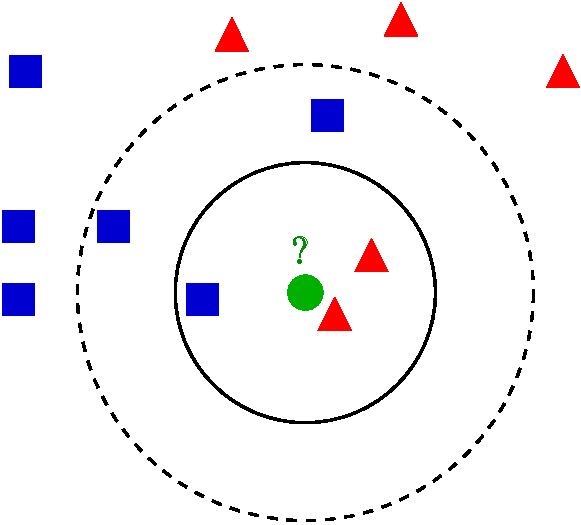
\includegraphics[width=0.7\linewidth]{./figure/KnnClassification.pdf}
\end{center}
\tiny \vspace{-0.3cm}
\url{https://en.wikipedia.org/wiki/K-nearest\_neighbors\_algorithm} \\ (CC-BY-SA 3.0; by Antti Ajanki)
\end{column}
\end{columns}
\end{block}
\end{frame}

\section{Proposed Method}
\label{sec:org4999f21}
\begin{frame}[label={sec:orge9985e4}]{Nearest Neighbor Machine Translation}
\begin{block}{Augmenting the decoder of a pre-trained NMT model with a nearest neighbor retrieval at each time step}
\begin{center}
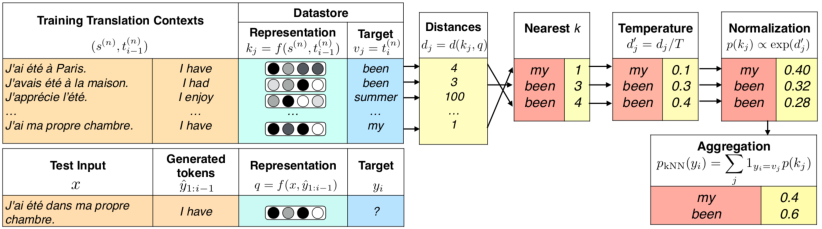
\includegraphics[width=0.8\linewidth]{./figure/Figure1.pdf}
\end{center}
\vspace{-0.3cm}
\begin{description}
\item[{Datastore:}] Datastore is constructed from parallel corpus by a single forward pass over each example.
\item[{\(q = f(x, \hat{y}_{1:i-1})\) :}] an intermediate representation of the decoder
\end{description}
\end{block}
\end{frame}

\begin{frame}[label={sec:org882ee60}]{Nearest Neighbor Machine Translation}
\vspace{-0.2cm}
\begin{center}
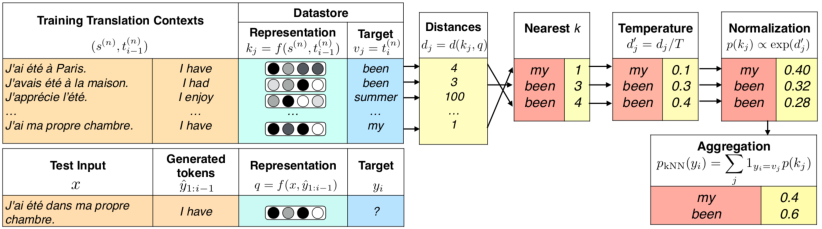
\includegraphics[width=0.75\linewidth]{./figure/Figure1.pdf}
\end{center}
\metroset{block=fill}
\renewcommand{\baselinestretch}{1.0}
\small
\vspace{-0.1cm}
\begin{block}{At test time}
\setlength{\parskip}{0.1em}
\begin{enumerate}
\item Search \(k\) nearest neighbors from the datastore based on distances between \(q\) and each intermediate representation.  \setlength{\itemsep}{0em}
\item Compute the distribution by applying a softmax with temperature to each \(k\) nearest neighbors.
\item Aggregate the 2. results and obtain probability \(p_{kNN}(y_i)\) .
\item Interpolate the NMT and kNN distribution.
\vspace{-0.3cm}
\end{enumerate}
\end{block}
\end{frame}

\begin{frame}[label={sec:org64ebb52}]{Datastore creation}
\begin{block}{Store the entire translation context, preliminarily}
\begin{equation*}
  (\highlight[orange]{$\mathcal{K}$},\highlight[mLightGreen]{$\mathcal{V}$}) = \{ (\highlight[orange]{$f(s, t_{1:i-1})$}, \highlight[mLightGreen]{$t_i$}), \forall t_i \in t \mid (s, t) \in (\mathcal{S}, \mathcal{T}) \} 
\end{equation*}
\begin{itemize}
\item \(f\) : NMT model (returns the decoder's intermediate representations)
\item \((\mathcal{S}, \mathcal{T})\) : parallel corpus
\item \highlight[orange]{ $\mathcal{K}$ : intermediate representations}, \highlight[mLightGreen]{ $\mathcal{V}$ : target tokens $t_i$}
\begin{itemize}
\item Conditioning on the source is implicit via the keys
\item The values are only target language tokens
\end{itemize}
\end{itemize}
\end{block}
\end{frame}

\begin{frame}[label={sec:org7bd30fc}]{Generation}
\small
\begin{block}{Compute distance-based probability distribution by applying a softmax with temperature}
\begin{equation*}
  \highlight[cyan]{$p_{kNN}(y_i | x, \hat{y}_{1:i-1})$} \propto \sum_{(k_j, v_j) \in \mathcal{N}} \mathbbm{1}_{y_i = v_j} \exp \left( \frac{ \highlight[orange]{$-d(k_j, f(x, \hat{y}_{1:i-1}))$} }{T} \right)
\end{equation*}
\begin{itemize}
\item \(\hat{y}\) : generated tokens \\
\item \(\mathcal{N}\) : \(k\) nearest neighbors according to squared-$L^2$ distance
\end{itemize}
\end{block}

\begin{block}{Interpolate with the NMT output distribution}
\begin{equation*}
  p(y_i | x, \hat{y}_{1:i-1}) = \lambda \highlightcap[cyan]{$p_{kNN}(y_i | x, \hat{y}_{1:i-1})$}{\footnotesize kNN distribution} + (1 - \lambda) \highlightcap[mLightGreen]{$p_{MT}(y_i | x, \hat{y}_{1:i-1})$}{\footnotesize NMT distribution}
\end{equation*}
\end{block}
\end{frame}

\begin{frame}[label={sec:org1970d26}]{Experimental Setup}
\begin{block}{NMT Model}
\begin{itemize}
\item Transformer big (\texttt{Fairseq})
\end{itemize}
\end{block}
\begin{block}{Tasks}
\begin{itemize}
\item WMT19 De-En news translation
\item Multilingual MT
\begin{itemize}
\item train: CCMatrix
\item test: newstest2018, newstest2019, TED Talks
\end{itemize}
\item Domain adaptation:
\begin{itemize}
\item Medical, Law, IT, Koran, Subtitles
\end{itemize}
\end{itemize}
\end{block}
\end{frame}

\begin{frame}[label={sec:org275f49f}]{Experimental Setup}
\begin{block}{Implementation of kNN-MT}
\begin{itemize}
\item kNN: \texttt{Faiss} (a library for fast k nearest neighbors search)
\item Key: 1024-dimensional input to the final decoder layer FFN \\ (quantized to 64-bytes)
\begin{itemize}
\item Multilingual MT:  131K clusters
\item Domain adaptation:  4K clusters
\end{itemize}
\item Inference: Query the datastore for 64 neighbors while searching 32 clusters
\end{itemize}
\end{block}
\end{frame}

\begin{frame}[label={sec:org04edca3},t]{Computational Cost}
\begin{block}{kNN-MT adds some computational overhead}
\metroset{block=fill}
\begin{columns}
\begin{column}[t]{0.5\columnwidth}
\begin{block}{Datastore creation}
\begin{itemize}
\item A single forward pass over all examples
\begin{itemize}
\item Same as one epoch
\end{itemize}
\end{itemize}
\end{block}
\end{column}
\begin{column}[t]{0.5\columnwidth}
\begin{block}{Inference}
\begin{itemize}
\item Retrieving 64 keys from a datastore containing billions of items
\item A generation speed that is two orders of magnitude slower than the base MT system
\end{itemize}
\end{block}
\end{column}
\end{columns}
\end{block}
\end{frame}

\begin{frame}[label={sec:org598022f}]{Experiments}
\begin{block}{WMT'19 De-En}
\begin{center}
\begin{tabular}{ll}
\toprule
Model & BLEU (\%)\\
\midrule
Baseline & 37.59\\
+kNN-MT & \textbf{39.08 (+1.5)}\\
\bottomrule
\end{tabular}
\end{center}

\begin{itemize}
\item Improving by 1.5 BLEU \% w/o additional training
\end{itemize}
\end{block}
\end{frame}

\begin{frame}[label={sec:org32172a4}]{Multilingual Machine Translation}
\begin{block}{Retrieving neighbors from same source language data}
\begin{center}
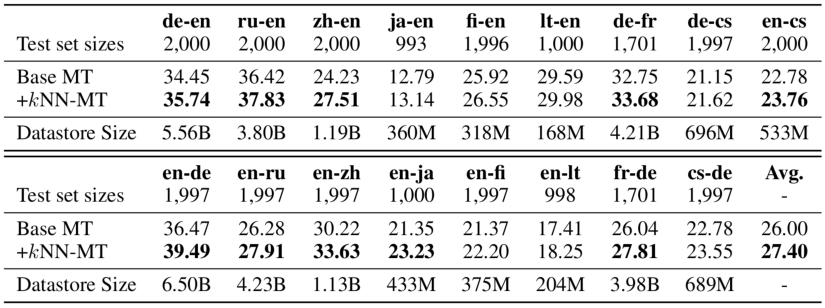
\includegraphics[width=\linewidth]{./figure/Table1.pdf}
\end{center}
\end{block}
\end{frame}

\begin{frame}[label={sec:orgd3555a9}]{Multilingual Machine Translation}
\begin{block}{Retrieving neighbors using English as the source language}
\begin{center}
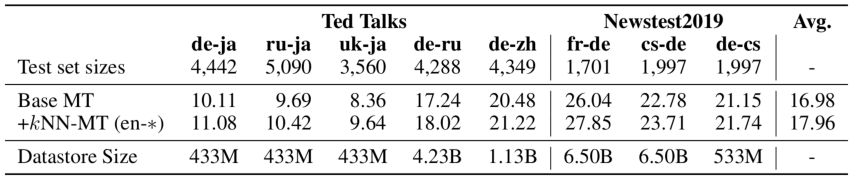
\includegraphics[width=\linewidth]{./figure/Table2.pdf}
\end{center}
\end{block}
\end{frame}

\begin{frame}[label={sec:orgfa60f73}]{Domain Adaptation}
\begin{block}{Domain-specific, out-of-domain, and multi-domain datastores}
\begin{center}
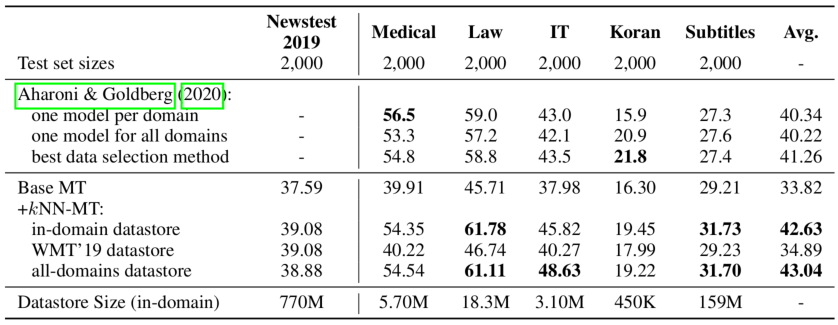
\includegraphics[width=\linewidth]{./figure/Table3.pdf}
\end{center}
\end{block}
\end{frame}

\begin{frame}[label={sec:org24739ce}]{Tuning kNN-MT (on validation set)}
\begin{block}{\# of neighbors per query \(k\)}
\begin{itemize}
\item \(k = 64\) (the \# of neighbors retrieved per query)
\item \textit{``we find that performance does not improve when retrieving a larger number of neighbors, and in some cases, performance deteriorates.''} (noise?)
\end{itemize}
\end{block}

\begin{block}{Softmax temperature \(T\)}
\begin{columns}
\begin{column}{0.5\columnwidth}
\begin{itemize}
\item \(T\) greater than 1 will
\begin{itemize}
\item flatten the distribution
\item increase diversity
\end{itemize}
\end{itemize}
\end{column}
\begin{column}{0.4\columnwidth}
\begin{textblock*}{\linewidth}(220pt, 125pt)
 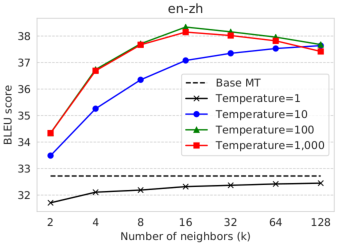
\includegraphics[width=\linewidth]{./figure/Figure2.pdf}
\end{textblock*}
\end{column}
\end{columns}
\end{block}
\end{frame}


\begin{frame}[label={sec:orge7c05ab}]{Tuning kNN-MT (on validation set)}
\begin{block}{Datastore size}
\begin{center}
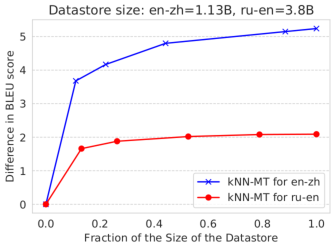
\includegraphics[width=0.5\linewidth]{./figure/Figure3.pdf}
\end{center}
\end{block}
\end{frame}

\begin{frame}[label={sec:org31ce93f}]{Qualitative Analysis}
\vspace{-0.2cm}
\begin{block}{Generate w/ only the kNN distribution ( \(\lambda = 1\) )}
\vspace{-0.5cm}
\begin{center}
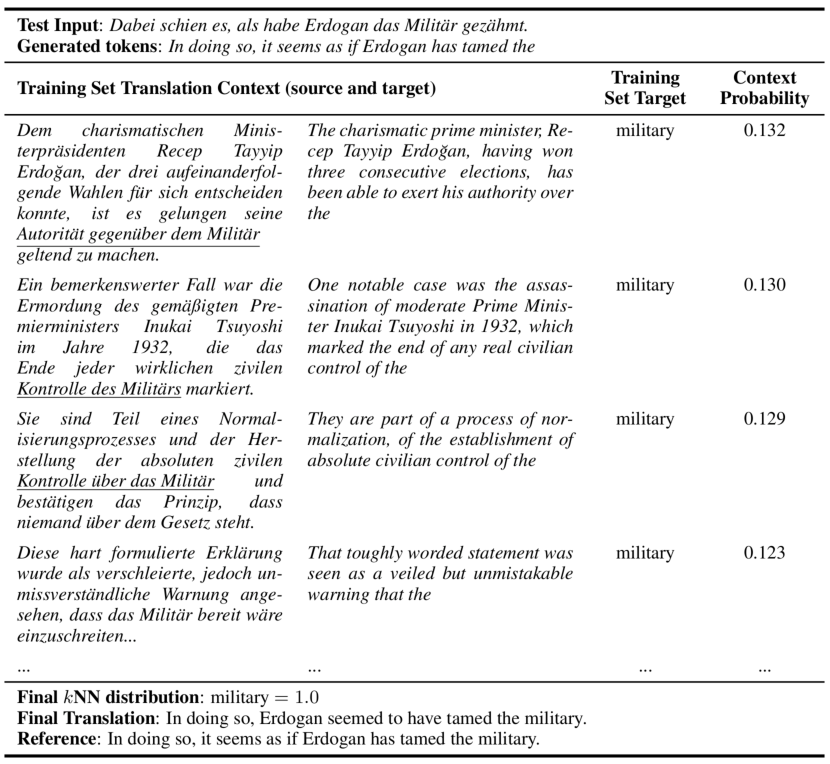
\includegraphics[width=0.5\linewidth]{./figure/Figure4.pdf}
\end{center}
\end{block}
\end{frame}

\section{Related Work}
\label{sec:org014ddbf}
\begin{frame}[label={sec:org88e5867}]{Example-Based Machine Translation (EBMT)}
\begin{block}{\small A Framework of a mechanical translation between Japanese and English by analogy principle \mycite{nagao-1984-framework}}
\begin{itemize}
\item e.g. English-to-Japanese bilingual corpus
\begin{center}
\footnotesize
\begin{tabular}{ll}
\toprule
English & Japanese\\
\midrule
Chick Corea is a fantastic \textbf{jazz pianist}. & チックコリアは素晴らしい\textbf{ジャズピアニスト}です。\\
Chick Corea is a fantastic \textbf{composer}. & チックコリアは素晴らしい\textbf{作曲家}です。\\
\bottomrule
\end{tabular}
\end{center}
\vspace{1em} EBMT system learns three units from the above example:
\begin{enumerate}
\item ``\textit{Chick Corea is a fantastic $\mathcal{X}$.}'' → ``\textit{チックコリアは素晴らしい $\mathcal{X}$ です。}''
\item ``\textit{jazz pianist}'' → ``\textit{ジャズピアニスト}''
\item ``\textit{composer}'' → ``\textit{作曲家 }''
\end{enumerate}
\end{itemize}
\end{block}
\end{frame}


\begin{frame}[label={sec:org6ad8692}]{Incorporating retrieval mechanisms into NMT}
\begin{block}{\small Guiding Neural Machine Translation with Retrieved Translation Pieces \mycite{zhang-etal-2018-guiding}}
\vspace{-0.3cm}
\begin{center}
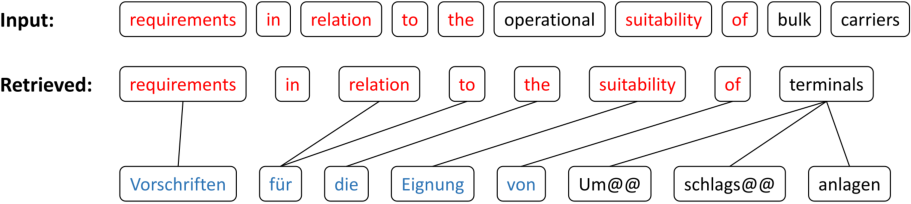
\includegraphics[width=0.8\linewidth]{./figure/zhang-etal-2018-guiding/Figure1.pdf}
\end{center}

\begin{columns}
\begin{column}{0.6\columnwidth}
\vspace{-1cm}
\begin{itemize}
\item Retrieve translation pieces (n-gram) of word-aligned parallel corpus
\item Add rewards for n-grams that occur in the collected translation pieces
\end{itemize}
\end{column}
\begin{column}{0.4\columnwidth}
\vspace{-0.6cm}
\begin{center}
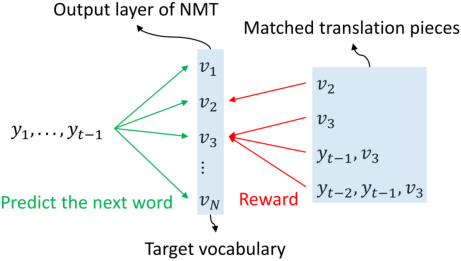
\includegraphics[width=\linewidth]{./figure/zhang-etal-2018-guiding/Figure2.pdf}
\end{center}
\end{column}
\end{columns}
\end{block}
\end{frame}

\begin{frame}[label={sec:org824430b}]{Retrieving translation examples}
\begin{block}{\small Search Engine Guided Neural Machine Translation \mycite{gu-etal-2018-search}}
\begin{itemize}
\item Retrieve examples similar to the test source sentence
\item Incorporate retrieved information w/ \textit{deep fusion / shallow fusion}
\end{itemize}

\vspace{-0.6cm}
\begin{center}
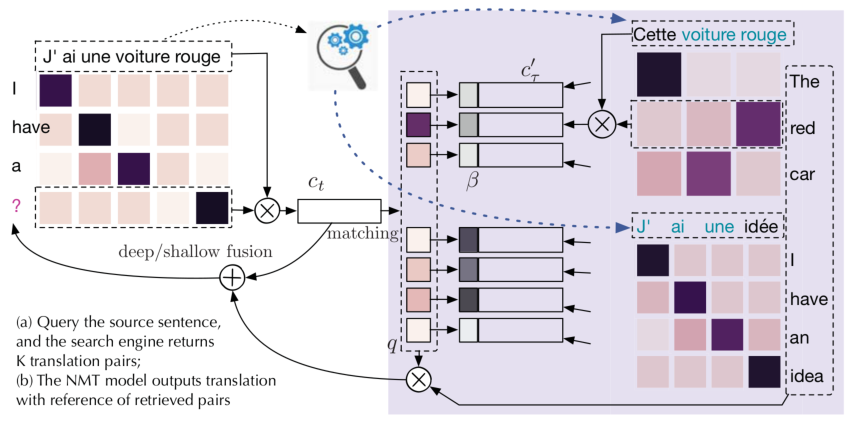
\includegraphics[width=0.75\linewidth]{./figure/gu-etal-2018-search/Figure1.pdf}
\end{center}
\end{block}
\end{frame}

\begin{frame}[label={sec:orge8cb6c3}]{Augumenting source sequences with retrieved translations}
\vspace{-0.3cm}
\begin{block}{\footnotesize Neural Fuzzy Repair: Integrating Fuzzy Matches into Neural Machine Translation \mycite{bulte-tezcan-2019-neural}}
\vspace{-0.1cm}
\begin{itemize}
\item Retrieve from translation memories by using edit distance based fuzzy-matching
\item Augment source sequences with retrieved translations
\begin{itemize}
\item e.g. ``\textit{こんにちは}'' → ``\textit{こんにちは || hi || good evening || have a nice day}''
\begin{itemize}
\item || : break token
\end{itemize}
\end{itemize}
\end{itemize}

\vspace{-0.3cm}
\end{block}
\begin{block}{\small Boosting Neural Machine Translation with Similar Translations \mycite{xu-etal-2020-boosting}}
\vspace{-0.1cm}
\begin{itemize}
\item Improvement of ``Neural Fuzzy Repair'' \mycite{bulte-tezcan-2019-neural}
\begin{itemize}
\item New score functions
\begin{itemize}
\item N-gram matching score
\item Embedding-based score
\end{itemize}
\item Additional information
\begin{itemize}
\item source tag, related target tag, un-related target tag, etc.
\end{itemize}
\end{itemize}
\end{itemize}
\end{block}
\end{frame}

\begin{frame}[label={sec:org57beabb}]{\small Learning to Remember Translation History with a Continuous Cache \mycite{tu-etal-2018-learning}}
\begin{block}{Saving and retrieving translation histories}
\begin{itemize}
\item Proposed model awares cross-sentence context in documents to prevent translation inconsistency.
\end{itemize}

\begin{center}
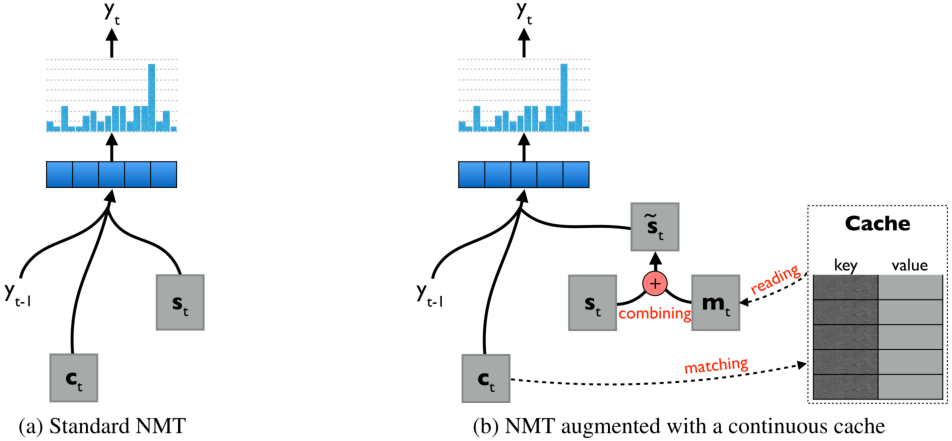
\includegraphics[width=0.7\linewidth]{./figure/tu-etal-2018-learning/Figure2.pdf}
\end{center}
\end{block}
\end{frame}

\begin{frame}[label={sec:org9d97adc}]{Conclusion}
\begin{block}{Summary}
\begin{itemize}
\item kNN-MT can apply to any NMT model w/o further training.
\item Similar contexts in a model's embedding space are more likely to be followed by similar next words, allowing the model to be improved by interpolation w/ kNN classifier.
\item kNN-MT improves a SOTA model in-domain, leads to large gains out-of-domain, and can specialize a multilingual model for specific language-pairs.
\end{itemize}

\vspace{-0.3cm}
\end{block}
\begin{block}{Future work}
\begin{itemize}
\item Improving efficiency
\begin{itemize}
\item e.g. Down-sampling frequent target words in the datastore
\end{itemize}
\end{itemize}
\end{block}
\end{frame}
\end{document}